\section{Gestión y Seguimiento del Proyecto en Jira}

Para la gestión y el seguimiento del desarrollo, el proyecto «Doble M» se organiza en Jira mediante un tablero Scrum. El flujo evoluciona de forma ágil a través de las columnas del sprint (\textit{Por hacer}, \textit{Asignado}, \textit{En curso}, \textit{En revisión} y \textit{Finalizado}), lo que permite ver el avance de las Historias de Usuario y subtareas en cada iteración.

El acceso al tablero oficial del proyecto se realiza a través del siguiente enlace: 
\url{https://go-team-yudm9r0y.atlassian.net/}

% ------------ PRIMERA IMAGEN: VISTA GENERAL DEL TABLERO JIRA ------------
\begin{figure}[htbp]
    \centering
    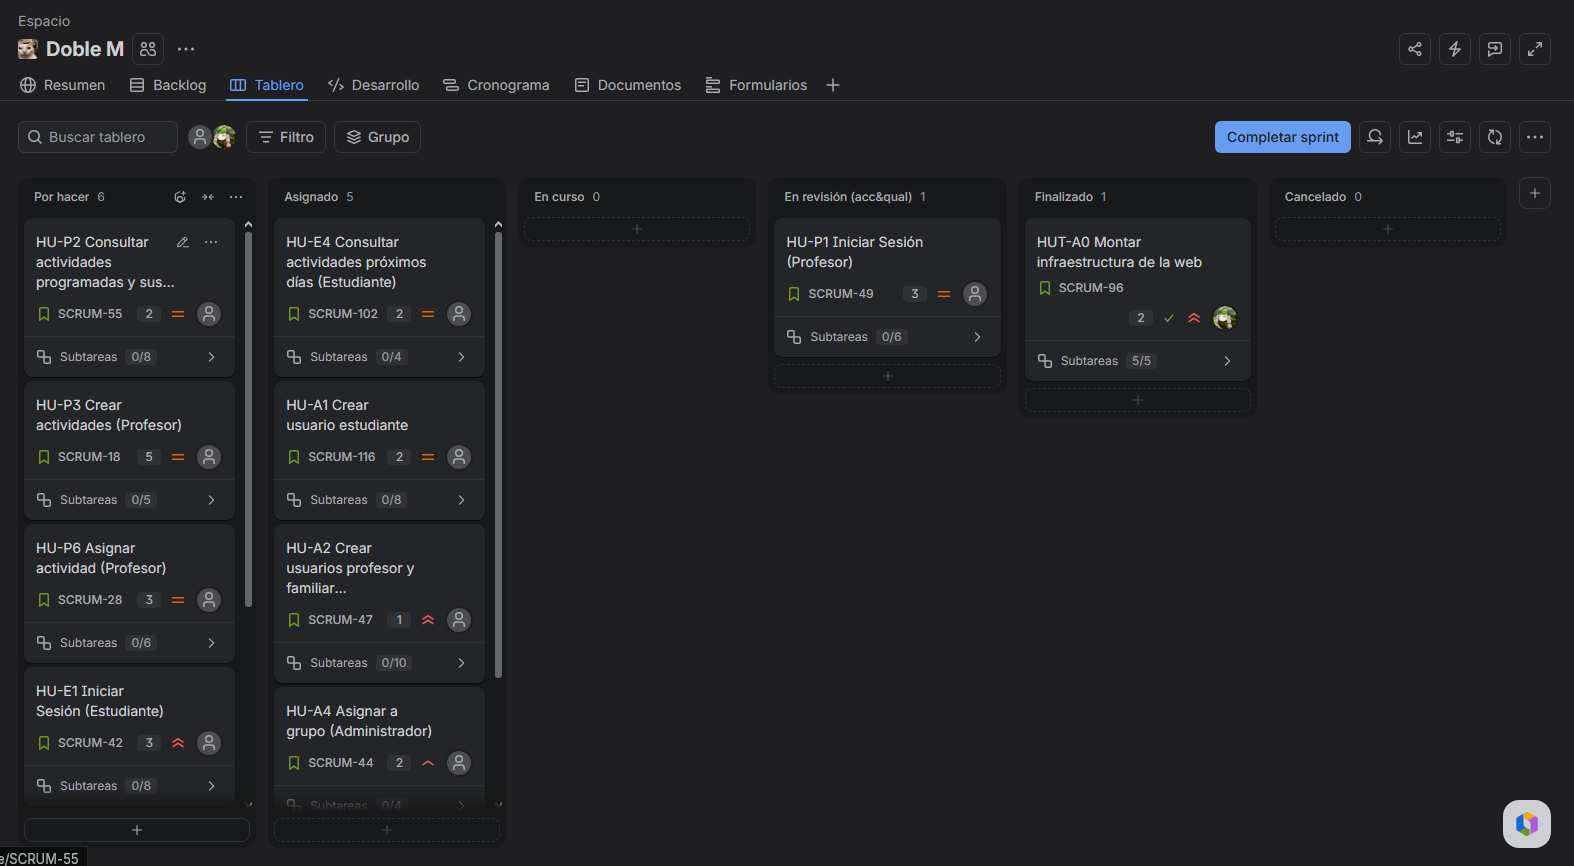
\includegraphics[width=1.1\textwidth]{img/primeraiteracion/jira1.png}
    \caption{Vista general del tablero Scrum en Jira para el proyecto Doble M.}
    \label{fig:jira_tablero_1}
\end{figure}

% ------------ SEGUNDA IMAGEN: DETALLE DEL SPRINT Y HISTORIAS ------------
\begin{figure}[htbp]
    \centering
    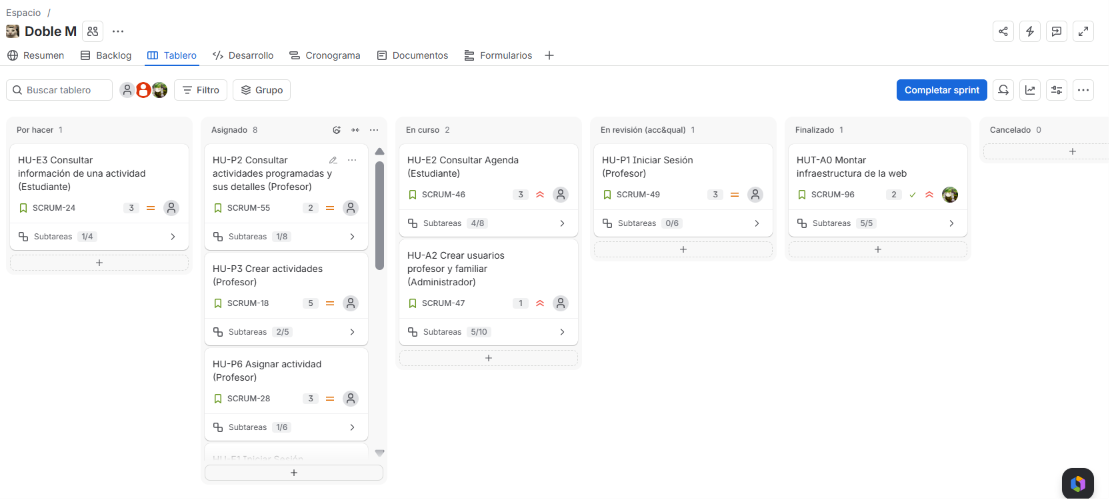
\includegraphics[width=1.2\textwidth]{img/primeraiteracion/jira2.png}
    \caption{Flujo de trabajo y estado de las Historias de Usuario en el sprint actual.}
    \label{fig:jira_tablero_2}
\end{figure}